\documentclass[10pt, oneside]{amsart}
\pagestyle{plain}
\usepackage{parskip, graphicx, amssymb, amsmath, epstopdf, enumitem, amsthm, pgfplots, tikz, tcolorbox, caption, subcaption, multicol}
\usepackage[all,cmtip]{xy}
\usepackage[mathscr]{euscript}
\DeclareGraphicsRule{.tif}{png}{.png}{`convert #1 `dirname #1`/`basename #1 .tif`.png}
\usetikzlibrary{shapes.geometric}

    
\newtheorem{thm}{Theorem}

\setlength{\tabcolsep}{20pt}
\renewcommand{\arraystretch}{1.5}

\textheight 642pt
\footskip 35pt
\voffset = -40pt
\addtolength{\oddsidemargin}{-.25in}
\addtolength{\textwidth}{0.5in}

\begin{document}

{\bf Math 1271 - Worksheet 16} \hfill \emph{11/5/2026}

{\bf\Large 3.3 - Local Max/Mins}

\medskip


\begin{enumerate}[leftmargin=0pt]

\item[1.] Suppose that $g(x)$ is a function that is continuous at every value of $x$ except at $x=2$. You may assume that this is because $g$ has a vertical asymptote at $x=2$. 

You may also assume that the \textbf{first derivative} of $g$ is
$$g'(x)=\dfrac{(x+4)(x-1)^2}{(x-2)}$$

\begin{enumerate}

\item[(a)] Determine all critical numbers of $g$.

\vspace{2.5in}

\item[(b)] By developing a carefully labeled first derivative sign chart, decide whether $g$ has a local minimum, local maximum, or neither at each critical number.

\vfill

\newpage

\item[(c)] Which of the following graphs is a possible graph of $y=g(x)$?

\bigskip

\begin{enumerate}

\item[(i)] \; 

\vspace{-25pt} 

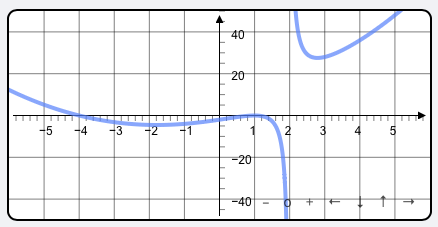
\includegraphics[scale=0.65]{wkst16option1-f25}

\bigskip

\item[(ii)] \; 

\vspace{-25pt} 

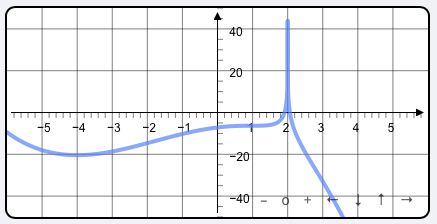
\includegraphics[scale=0.65]{wkst16option2-f25}

\bigskip

\item[(iii)] \; 

\vspace{-25pt} 

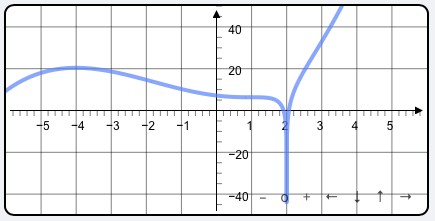
\includegraphics[scale=0.65]{wkst16option3-f25}

\bigskip

\item[(iv)] \; 

\vspace{-25pt} 

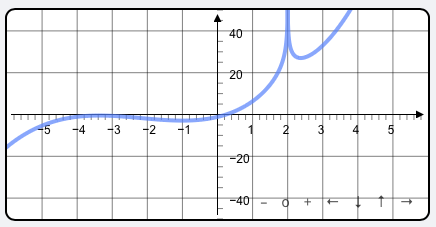
\includegraphics[scale=0.65]{wkst16option4-f25}

\end{enumerate}

\end{enumerate}

\bigskip

\newpage



\item[2.] 

\begin{enumerate}

\item[(a)] Let $f(x)=x^4(x-1)^3$. 

\begin{enumerate}

\item[(i)] The function $f$ has three critical numbers; find them. 

\vfill

\item[(ii)] You may assume that
$$f''(x)=6x^2(x-1)(7x^2-8x+2)$$
What does the Second Derivative Test tell you about the critical numbers you found in part (a)?

\vfill

\item[(iii)] What does the First Derivative Test tell you about the critical numbers you found in part (a)?

\vfill

\end{enumerate}

\newpage

\item[(b)] Let $g(t)=t^2\ln(t)$. 

\begin{enumerate}

\item[(i)] The function $g$ has one critical number; what is it?

\vfill

\item[(ii)] Is this critical number a local maximum of $g$, a local minimum of $g$, or neither one?

\vfill

\end{enumerate}

\end{enumerate}

\newpage


\item[3.] Suppose that $g$ is a function whose \textbf{second derivative}, $g''$, is given by the graph below:

\begin{center}
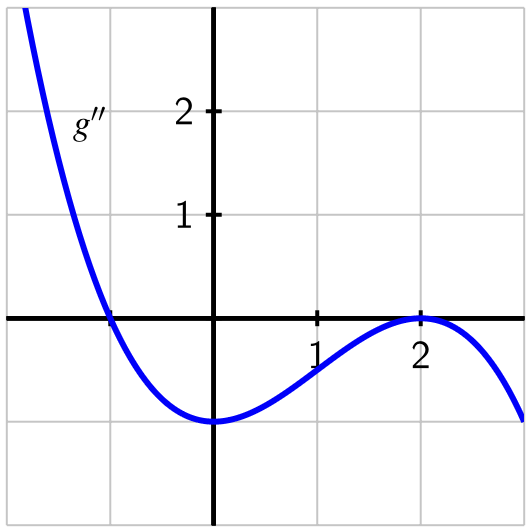
\includegraphics[scale=0.3]{wkst16graph-f25}
\end{center}

\begin{enumerate}

\item[(a)] Find the $x$-coordinates of all points of inflection of $g$.

\vfill

\item[(b)] Suppose you are given that $g'(-1.67857351)=0$. Is there a local maximum, local minimum, or neither (for the function $g$) at this critical point, or is it impossible to say?

\vfill

\item[(c)] Assuming that $g''(x)$ is a polynomial (and that all important behavior of $g''(x)$ is seen in the graph above), what degree polynomial do you think $g(x)$ is? (Hint: Think about the Power Rule. How does the degree of a polynomial relate to the degree of its second derivative?)

\vfill

\end{enumerate}

\end{enumerate}

\end{document}  